\documentclass[11pt,a4paper]{article}
\usepackage[utf8]{inputenc}
\usepackage{graphicx}
\usepackage{titlesec}
\usepackage{hyperref}
\usepackage{fancyhdr}
\usepackage{mathptmx}
\usepackage[english]{babel}
\usepackage{amsmath}
\usepackage{subcaption}
\usepackage[svgnames]{xcolor}
\usepackage{tocloft}
\usepackage{pdfpages}
\usepackage{float}
\usepackage{enumitem}
\usepackage[table]{xcolor}
\usepackage{array}
\usepackage{xurl}
\usepackage{stfloats} 
\usepackage{xurl}
\urlstyle{tt}

% \usepackage[letterpaper, margin=0.8in]{geometry}
\usepackage[a4paper, left=1cm, right=1cm, top=2cm, bottom=2cm]{geometry}

\usepackage{etoolbox}
\usepackage{booktabs}
\usepackage{longtable}
\usepackage{pgfgantt}
\usepackage{multicol}
\usepackage{float}
\usepackage{setspace}
\usepackage{indentfirst}
\usepackage{enumitem} 


\usepackage{graphicx}
\usepackage{tabularx}
\usepackage[table]{xcolor} % For table colors
\usepackage{array}

\definecolor{aur_color}{RGB}{189, 13, 47}


% Formatting
\titleformat{\section}{\color{aur_color} \normalfont\LARGE\bfseries}{\thesection\quad}{0em}{}[\titlerule]
\titleformat{\subsection}{\color{aur_color} \normalfont\Large\bfseries}{\thesubsection\quad}{0em}{}
\titleformat{\subsubsection}{\normalfont\large\bfseries}{\thesubsubsection\quad}{0em}{}

% Hyperlink Setup
\hypersetup{
    colorlinks=true,
    linkcolor=blue,
    filecolor=magenta,   
    urlcolor=cyan,
    pdftitle={AU-Robotics Preliminary Design Review},
}

% Page Style
\pagestyle{fancy}
\fancyhf{}
\rhead{Preliminary Design Review}
\lhead{AU-Robotics}
\cfoot{\thepage}

% Document Start
\AtBeginDocument{
    \addtocontents{plain}{\protect\thispagestyle{plain}}
}

\begin{document}
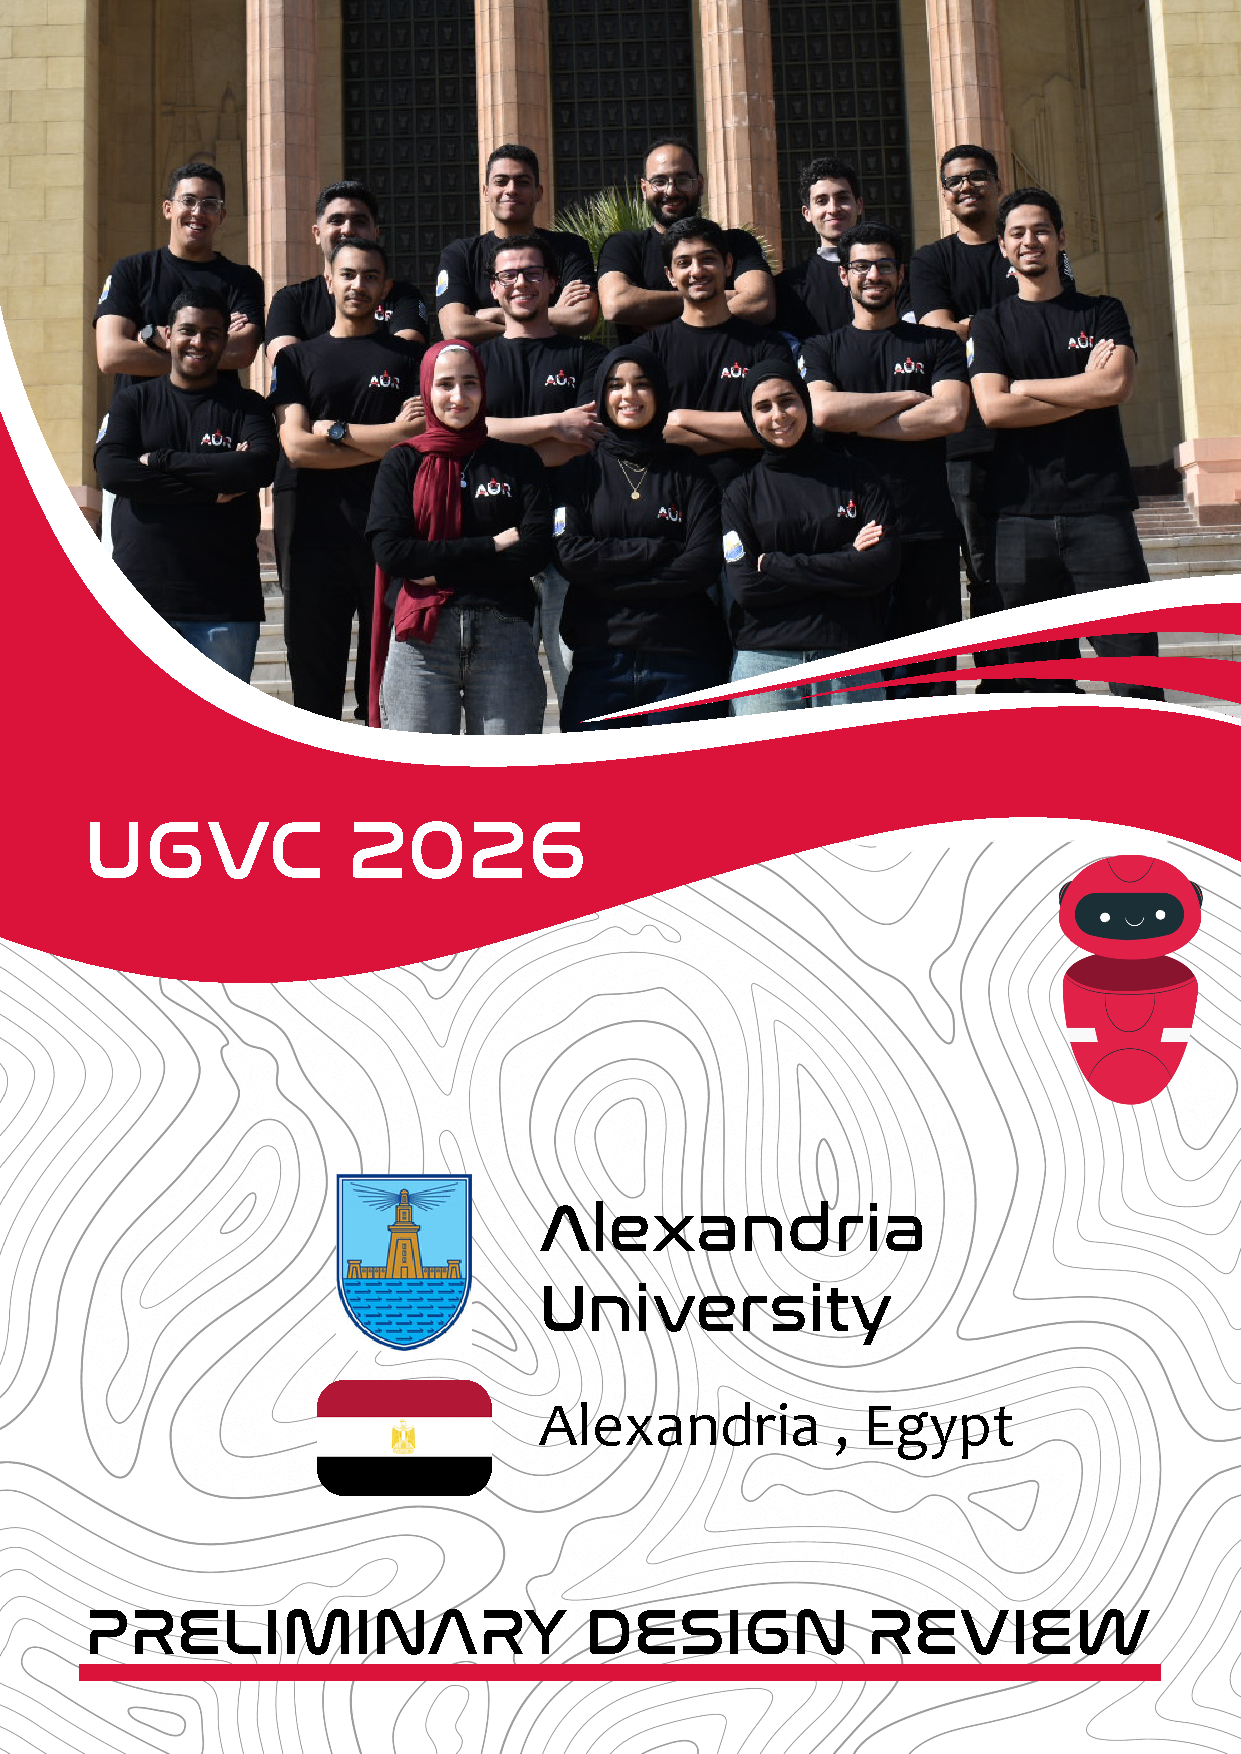
\includepdf[pages=-, fitpaper=true]{assets/cover.pdf}

\newpage

% \title{Preliminary Design Review (PDR)}
% \author{AU-Robotics}
% \date{\today}

% \renewcommand{\contentsname}{}  
% \maketitle
% \begin{center}
%     \Large \textbf{Table of Contents}
% \end{center}
% \begin{multicols}{2}
% \tableofcontents
% \end{multicols}

\setlength{\columnsep}{1.5cm}
\twocolumn
\section{ Team Structure}
The \textbf{AU-Robotics Team} at Alexandria University is a dedicated group of engineering students founded in 2021. Since its establishment, the team has participated in several robotics competitions including \textbf{Minesweepers}, \textbf{Micromouse}, \textbf{IEEE Victoris}, \textbf{IEEE Mutex}, and \textbf{ORCE}.

Our team follows a structured hierarchy to ensure an efficient workflow. The \textbf{Faculty Advisor} provides technical mentorship and guidance, while the \textbf{CEO} is responsible for overall coordination and strategic planning. The \textbf{CFO} manages financial matters, and the \textbf{CTO} supervises technical development and system integration. The team is divided into four main divisions, each led by a \textbf{Technical Head} who oversees the work of the subteam:
\vspace{-2pt}
\begin{itemize}[left=0pt] 
    \setlength{\itemsep}{0pt}
    \setlength{\parskip}{0pt}
    \setlength{\parsep}{0pt} 
    \item \textbf{Hardware:} Responsible for power systems and electronic components.
    \item \textbf{Mechanical:} Focuses on the robot chassis and drivetrain design.
    \item \textbf{Software:} Develops navigation and perception algorithms.
    \item \textbf{Firmware:} Handles low-level programming and communication with hardware.
\end{itemize}
\vspace{-3pt}

This structure enables clear task delegation and supports smooth and organized progress across the team’s projects.

% Each division has specialized sub-teams led by Hardware, Software, and Mechanical Leads, ensuring efficient development. 

\section{Vehicle Overview}

\subsection{Mechanical Design}
The rover is designed to achieve high maneuverability, stability, and mobility across grassy and uneven terrain while maintaining relatively high traversal speed. Additionally, the platform must support precise steering in confined environments, which requires a stable suspension system and reliable traction.

To satisfy these requirements, the rover employs a rocker-bogie suspension system combined with differential steering. This configuration provides excellent obstacle traversal capability, improved terrain adaptability, and continuous wheel contact with the ground.
% The mechanical design prioritizes durability, modularity, and competition compliance.

\begin{figure}[H]
        \centering
        
\includegraphics[width=\linewidth, height =3.85cm]{Rover_Assembly.jpeg}
        \caption{Primary Stage}
        \label{fig:primary_stage}
\end{figure}


\subsubsection{Frame Structure}
The rover frame serves as the primary structural backbone, supporting all mechanical and electronic subsystems including the suspension system, drivetrain components, batteries, sensors, and payload.
The structure is designed with a streamlined aerodynamic profile to minimize pressure drag during forward motion, thereby improving the rover’s overall energy efficiency.

The frame is constructed using aerospace-grade aluminum alloy, which provides an optimal balance between high strength, corrosion resistance, and low weight. This material selection ensures the structure can withstand harsh environmental conditions while maintaining structural integrity under operational loads.

\noindent\textbf{Frame Specifications:}
\begin{itemize}[left=0pt]
\setlength{\itemsep}{0pt}
\setlength{\parskip}{0pt}
\setlength{\parsep}{0pt}
\vspace{-7pt}
\item \textbf{Dimensions:}
    \begin{itemize}[left=0pt, label=-]
    \setlength{\itemsep}{0pt}
    \setlength{\parskip}{0pt}
    \setlength{\parsep}{0pt}
    \item Length: 150 cm
    \item Width: 80 cm
    \item Height: 110 cm
    \end{itemize}

\end{itemize}

The frame is designed to safely support a payload capacity of approximately \textbf{50 kg} while maintaining structural rigidity under both simulated and real-world operating conditions.


\subsubsection{Rocker-Bogie Suspension System} The rover utilizes a rocker-bogie suspension system, a configuration widely used in planetary exploration rovers due to its ability to maintain continuous wheel-ground contact across highly irregular terrain. The rocker-bogie assembly is fabricated from aluminum alloy sheet metal, offering a lightweight yet durable structure capable of withstanding extreme environmental and terrain conditions. This suspension system allows the rover to traverse a variety of terrains, including: \vspace{-7pt} \begin{itemize}[left=0pt, label=-] \setlength{\itemsep}{0pt} \setlength{\parskip}{0pt} \setlength{\parsep}{0pt} \item Dry rocky surfaces \item Uneven grassy environments \item Desert-like conditions \item Mud and loose soil (with appropriate wheel selection) \end{itemize} The rocker-bogie mechanism enables the rover to navigate obstacles across the three spatial axes (X, Y, and Z) while maintaining platform stability. This ensures smoother motion when climbing obstacles and reduces sudden chassis tilting.


\subsubsection{Traction System}

The traction system is designed to provide high torque for obstacle traversal while maintaining adequate speed for efficient terrain coverage.

The drivetrain uses a front and rear motor configuration, while the middle wheel primarily contributes to stability and climbing capability when the rover encounters obstacles.

Power transmission is achieved using a chain-and-sprocket drivetrain, which offers several advantages:


\vspace{-7pt}
\begin{itemize}[left=0pt, label=-]
\setlength{\itemsep}{0pt}
\setlength{\parskip}{0pt}
\setlength{\parsep}{0pt}
\item Reliable torque transmission
\item Efficient power delivery
\item Adjustable gear ratios for RPM optimization
\end{itemize}


This configuration allows the system to increase wheel rotational speed while preserving motor torque output.

The rover is equipped with 10-inch foam-filled tires, selected for their durability and reliability in hazardous terrain. Foam-filled tires eliminate the risk of punctures, ensuring continuous operation even in rough environments.

The propulsion system utilizes brushed DC motors rated at 120 RPM with a torque of approximately 80 kg·cm. These motors provide sufficient torque for obstacle traversal and off-road mobility.

When combined with the chain-and-sprocket transmission system, the rover achieves a maximum linear speed of approximately 10 km/h, balancing both high torque performance and efficient traversal speed.

\begin{table}[h]
\centering
\renewcommand{\arraystretch}{1.2}

\begin{tabularx}{\linewidth}{|l|X|}
\hline
\rowcolor{aur_color}
\textcolor{white}{Parameter} & \textcolor{white}{Specification} \\ \hline

Suspension System & Rocker-Bogie \\ \hline
Steering Method & Differential Steering \\ \hline
Frame Material & Aerospace-grade Aluminum Alloy \\ \hline
Payload Capacity & 50 kg \\ \hline
Wheel Diameter & 10 inch Foam-Filled Tires \\ \hline
Motors & Brushed DC Motors \\ \hline
Motor Speed & 120 RPM \\ \hline
Motor Torque & 80 kg·cm \\ \hline
Transmission & Chain and Sprocket Drive \\ \hline
Maximum Linear Speed & 10 km/h \\ \hline

\end{tabularx}

\caption{System Specifications}
\label{tab:specs}

\end{table}


\vspace{-7pt}
\subsection{Hardware}

\subsubsection{Power system}
 The power system utilizes Lithium Polymer (LiPo) cells in a series-parallel configuration to achieve a nominal output of \textbf{24V} while meeting the robot's capacity requirements. To distribute power safely across subsystems, a dual-stage regulation strategy is implemented:
 \begin{itemize}[left=0pt] 
    \setlength{\itemsep}{0pt}
    \setlength{\parskip}{0pt}
    \setlength{\parsep}{0pt} 
    \item \textbf{Primary Stage:} An \textbf{LM2576HVS-ADJ} buck regulator steps down the main 24V bus to a \textbf{12V} rail.
    \begin{figure}[H]
        \centering
        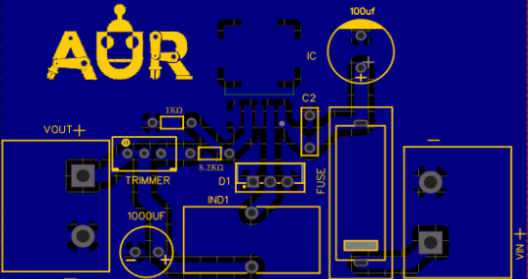
\includegraphics[width=\linewidth]{assets/primary_stage.png}
        \caption{Primary Stage}
        \label{fig:primary_stage}
    \end{figure}
    

    \item \textbf{Secondary Stage:} An \textbf{XL4015E1} high-efficiency DC-DC converter further reduces the \textbf{12V} supply to a stable \textbf{5V} rail for MCU, logic and sensor components. This hierarchical approach ensures voltage stability and protects sensitive electronics from fluctuations.

        \begin{figure}[H]
        \centering
        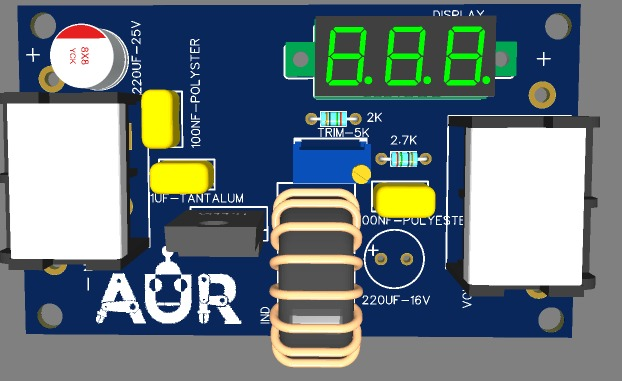
\includegraphics[width=\linewidth]{assets/secondary_stage.jpg}
        \caption{Secondary Stage}
        \label{fig:secondary_stage}
    \end{figure}


\end{itemize}


\subsubsection{Main board}

The Main Control Board serves as the central integration hub for the robot’s electronics. It houses the  microcontroller, which manages real-time tasks and provides high-level connectivity. This board facilitates seamless communication with the Raspberry Pi for computationally intensive operations. Furthermore, the PCB provides dedicated interfaces for critical peripherals, including the GPS module for localization and the lighting system for status indication and illumination.

\subsubsection{Motor control}
The motor actuation system is driven by a custom-engineered H-bridge circuit utilizing IR2104PBF half-bridge gate drivers and IRLZ44N Logic-Level N-Channel MOSFETs. To ensure high-speed switching and thermal stability, we implemented a dedicated Motor Control Board featuring a secondary  microcontroller. This modular approach provides total electrical isolation from the main board and allows for real-time motor processing. The motor-specific MCU communicates directly with the Raspberry Pi, ensuring low-latency execution of movement commands.

\begin{figure}[H]
    \centering
    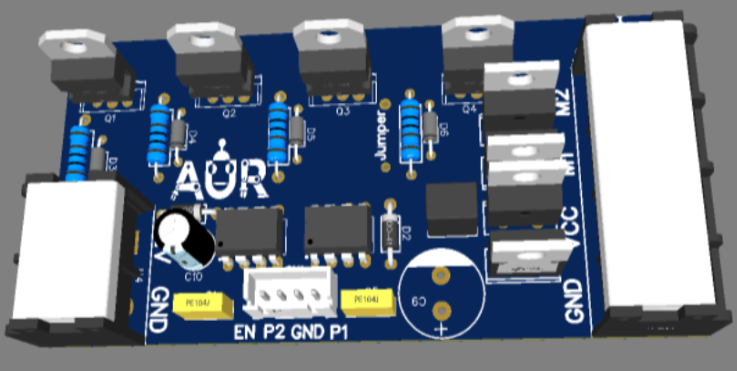
\includegraphics[width=\linewidth]{assets/Motor_Contol_Board.png}
    \caption{Motor Contol Board}
    \label{fig:placeholder}
\end{figure}

% as shown in the figure below.

% \begin{figure}[h!]
%     \centering
%     \includegraphics[width=0.3\textwidth]{hw.jpeg}
%     \caption{H-Bridge Circuit.}
%     \label{fig:system-architecture}
% \end{figure}




\subsection{Software}

\subsubsection{System Architecture}
The embedded subsystem runs on an STM32 microcontroller and is responsible for low-level hardware control and sensor data acquisition. It communicates with the Raspberry Pi over USB CDC. The Raspberry Pi serves as the main compute platform, running ROS2 and hosting both third-party and custom packages. All sensing, navigation, and control logic is coordinated through the ROS2 topic system.

Our ROS2 system uses three ready-made packages for autonomous navigation and three custom packages to complete the architecture, as shown in the figure.
\begin{figure}[H]
    \centering
    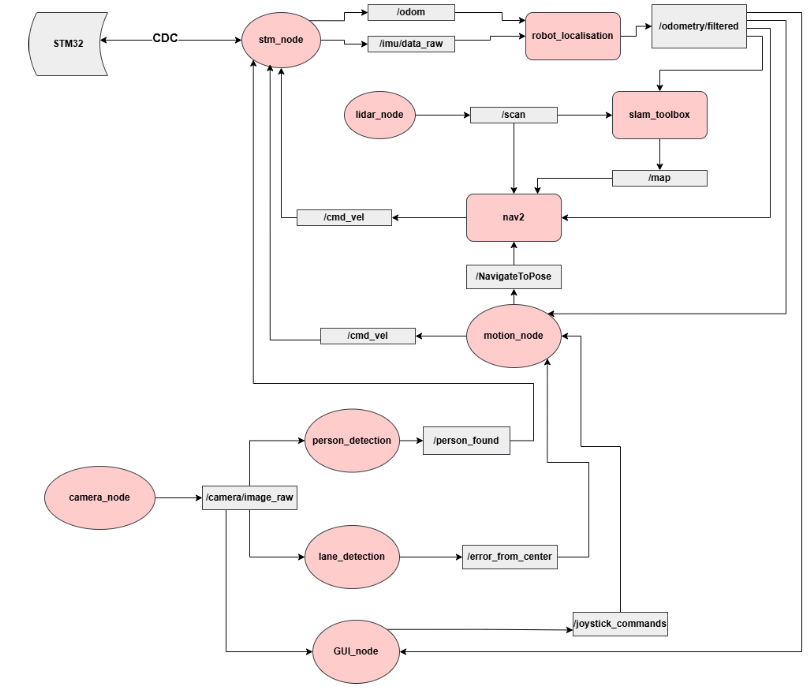
\includegraphics[width=\linewidth]{assets/ROS2_system.png}
    \caption{ROS2 System}
    \label{fig:placeholder}
\end{figure}


For the ready-made packages, \path{robot_localization} fuses IMU and odometry into filtered odometry, \path{slam_toolbox} builds and maintains the map, and Nav2 handles path planning and obstacle avoidance.

On the custom side, \path{stm_node} bridges the STM32 over USB CDC, \path{person_detection} runs YOLO on the camera feed, \path{lane_detection} uses computer vision to compute the lane deviation, and the GUI node forwards joystick inputs, all feeding into the \path{motion_node}, which arbitrates between all sources to publish the final \path{/cmd_vel}.


% \newpage
\section{Motion Control}

\subsection{Manual}

The rover supports manual operation through the GUI node, which receives joystick inputs and publishes \texttt{/joystick\allowbreak\_commands} to the \texttt{motion\_node}. The \texttt{motion\_node} translates these commands into \texttt{/cmd\_vel}, forwarded to the STM32 via \texttt{stm\_node} for direct motor control.

% The primary goal is to navigate within predefined paths, detect and avoid obstacles, and reach way points accurately while maintaining stability and efficiency.

\subsection{Autonomous Navigation}

The autonomous navigation system enables the rover to navigate outdoor cluttered environments independently, integrating localization, mapping, lane detection, and obstacle avoidance. To achieve this, the MPU9250 was chosen as our IMU to provide real-time orientation (yaw, pitch, roll), along with a LiDAR for 2D environment scanning and rotary encoders with 4× quadrature decoding for precise displacement, speed, and direction measurement.

\subsubsection{Localization \& Mapping}

The \texttt{robot\_localization} package fuses IMU and encoder data via EKF, producing filtered odometry on \texttt{/odometry/filtered}. \texttt{slam\_toolbox} then builds and maintains a real-time map using LiDAR scan data.

\subsubsection{Navigation Modes}

\begin{itemize}[left=0pt, label=-, itemsep=0pt, topsep=0pt]
\item Lane Following: lane centering using \path{/error_from_center} from the \path{lane_detection} node
\item Waypoint Navigation: rover navigates to a target pose via \path{/NavigateToPose}, with Nav2 handling path planning
\item Obstacle Avoidance: Nav2 dynamically replans when obstacles appear in the LiDAR scan
\end{itemize}



% Lane Detection
\section{Lane Detection \&\\Obstacle Avoidance}
The \texttt{lane\_detection} node determines the rover’s error from the center of the lanes by utilizing computer vision techniques such as edge detection and feature extraction demonstrated in figure.
\begin{figure}[H]
    \centering
    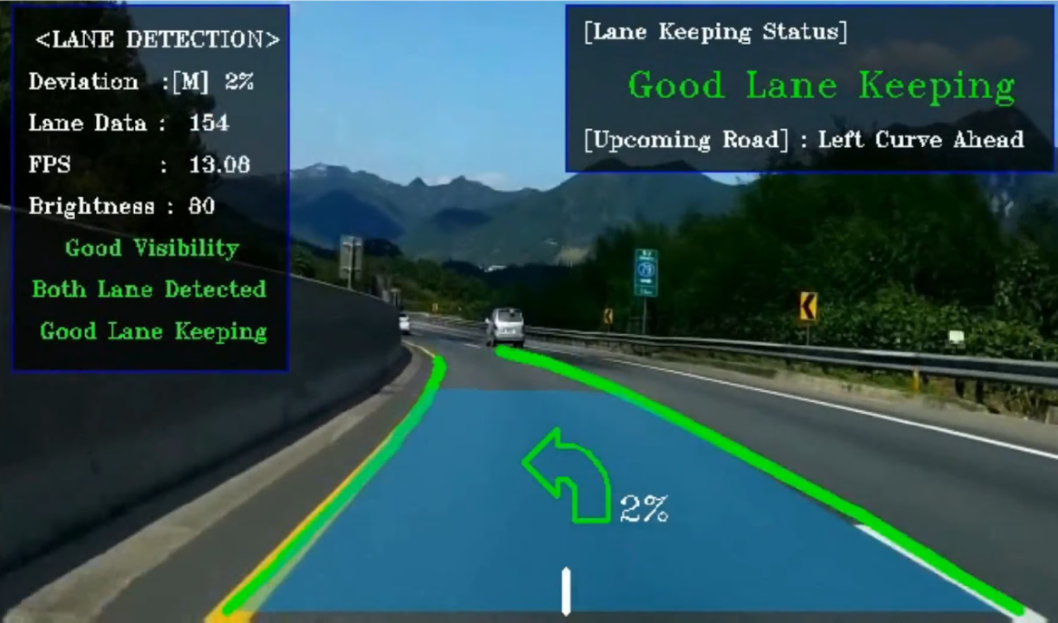
\includegraphics[width=\linewidth]{assets/lane_detection.png}
    \caption{Lane detection}
    \label{fig:placeholder}
\end{figure}



As a rudimentary technique for obstacle detection, the center calculation offsets the path taken on the short-term when an object is detected and is either hiding one of the two lanes or is showing two different-width passages. As shown in figure below, the rover knows to avoid the obstacle as it can sufficiently center itself between the obstacle and the left lane.
\begin{figure}[H]
    \centering
    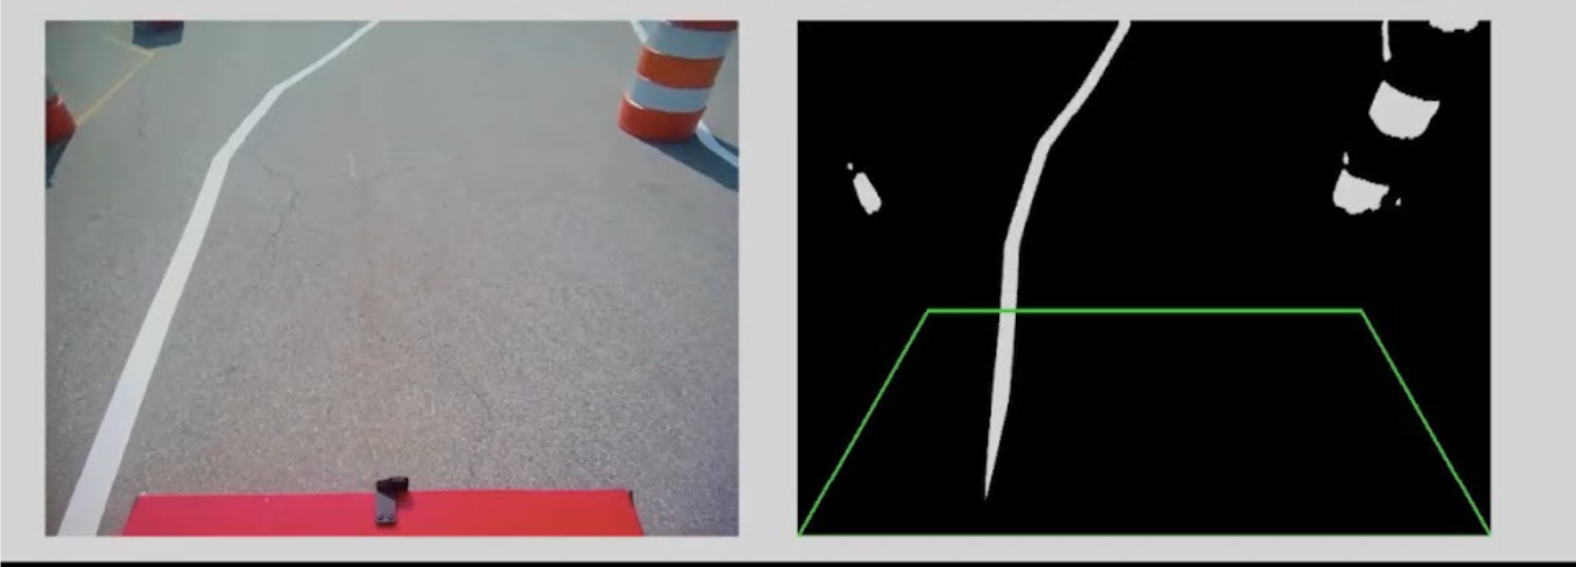
\includegraphics[width=\linewidth]{assets/obstacle_avoidance.png}
    \caption{Obstacle Avoidance}
    \label{fig:placeholder}
\end{figure}


\section{Project Management Plan}


\subsection{Development Plan}
Our development is structured into four key phases:
\vspace{-8pt}
\begin{itemize}
    \setlength{\itemsep}{0pt}
    \setlength{\parskip}{0pt}
    \setlength{\parsep}{0pt}
    \item \textbf{Planning \& Research:} Defining requirements, selecting components, and initial system design.
    \item \textbf{Design \& Implementation:} Mechanical assembly, electrical integration, and software development.
    \item \textbf{Testing \& Debugging:} System validation, sensor calibration, and refining navigation algorithms.
    \item \textbf{Final Refinement:} Performance optimization and competition preparation.
\end{itemize}
 

\vspace{12pt}
\subsection{Timeline}

The project follows a structured timeline to ensure timely completion.  
The table below presents the estimated schedule.

\begin{figure}[H]
\centering
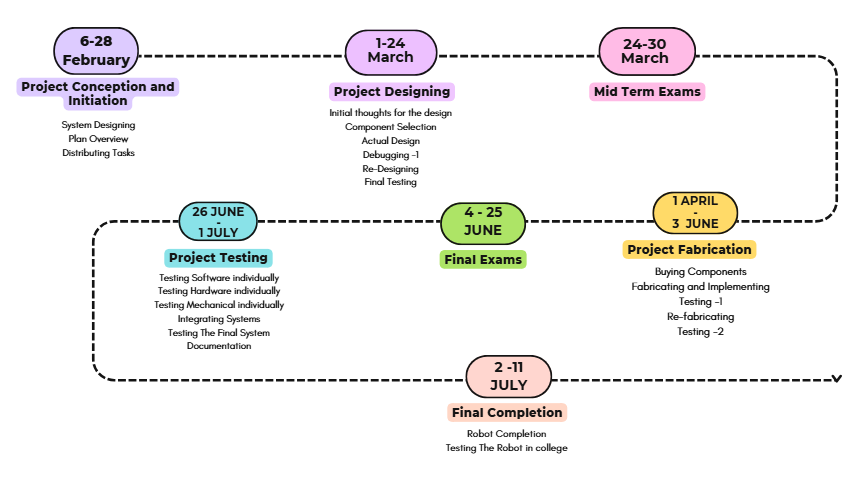
\includegraphics[width=\columnwidth]{assets/Timeline.png}
\caption{Rover Timeline}
\label{fig:timeline}
\end{figure}

\subsection{Budget}

\begin{flushright}
\small
\setlength{\tabcolsep}{4pt}

\begin{tabular}{|l|c|}
    \hline
    \rowcolor{aur_color}
    \textcolor{white}{\textbf{Mechanical System}} & \textcolor{white}{\textbf{Price (in EGP)}}\\
    \hline
    Chassis materials & \\
    Suspension & 32,000 \\
    Motors & \\
    Fabrication & \\
    \hline
    \rowcolor{aur_color}
    \textcolor{white}{\textbf{Electronics \& Sensors}} & \\
    \hline
    LiDAR & \\
    Cameras & 15,200 \\
    IMU & \\
    Microcontrollers & \\
    \hline
    \rowcolor{aur_color}
    \textcolor{white}{\textbf{Logistics \& Competition Fees}} & \\
    \hline
    Transport & \\
    Accommodation & 17,000 \\
    Registration fees & \\
    \hline
    \rowcolor{aur_color}
    \textcolor{white}{\textbf{Total}} & \textcolor{white}{64,200} \\
    \hline
\end{tabular}

\captionof{table}{Budget Breakdown}
\label{tab:budget}

\end{flushright}



\end{document}
